\documentclass[10pt]{article}
\usepackage{amsmath}
\usepackage{graphicx}
\usepackage[colorlinks=true,linkcolor=cyan,citecolor=magenta]{hyperref}
%\usepackage{showframe}

\title{A treatise on phenomenological models of surface second-harmonic
generation from crystalline surfaces}
\author{Bernardo S. Mendoza and Sean M. Anderson}
\date{\today}

\begin{document}
\maketitle
%\tableofcontents
%\pagebreak

\section{Three layer model for SHG radiation}

In this section we derive the formulas required for the calculation of the SHG
yield, defined by
\begin{equation*}\label{uno}
R(\omega)=\frac{I(2\omega)}{I^2(\omega)}
,
\end{equation*}
with the intensity
\begin{equation*}\label{dos}
I(\omega)=\frac{c}{2\pi}|E(\omega)|^2
,
\end{equation*}
There are several ways to calculate $R$, one of which is the procedure followed
by Cini \cite{ciniPRB91}. This approach calculates the nonlinear susceptibility
and at the same time the radiated fields. However, we present an alternative
derivation based in the work of Mizrahi and Sipe \cite{mizrahiJOSA88}, since
the derivation of the three-layer-model is straightforward. Within our level of
approximation this is the best model that we can use. In this scheme, we assume
that the SH conversion takes place in a thin layer, just below the surface,
that is characterized by a surface dielectric function
$\epsilon_{\ell}(\omega)$. This layer is below vacuum and sits on top of the
bulk characterized by $\epsilon_{b}(\omega)$ (see Fig. \ref{3layer}). The
nonlinear polarization immersed in the thin layer, will radiate an electric
field directly into vacuum and also into the bulk. This bulk directed field,
will be reflected back into vacuum. Thus, the total field radiated into vacuum
will be the sum of these two contributions (see Fig. \ref{3layer}). We
decompose the field into $s$ and $p$ polarizations, then the electric field
radiated by a polarization sheet,
\begin{align}\label{tres}
\mathcal{P}_i(2\omega)=\chi_{ijk}E_{j}(\omega)E_{k}(\omega)
,
\end{align}
is given by \cite{mizrahiJOSA88},
\begin{equation*}\label{r2}
(E_{p\pm},E_s) = 
(\frac{2\pi i\tilde{\omega}^2}{w}
\,\hat{\mathbf{p}}_\pm\cdot\boldsymbol{\mathcal{P}},
\frac{2\pi i\tilde{\omega}^2}{w}
\,\hat{\mathbf{s}}\cdot\boldsymbol{\mathcal{P}}),
\end{equation*}
where $\hat{\mathbf{s}}$ and $\hat{\mathbf{p}}_\pm$ are the unitary vectors for
$s$ and $p$ polarization, respectively, and the $\pm$ refers to upward ($+$) or
downward ($-$) direction of propagation. Also, $\tilde\omega=\omega/c$ and
$w_i=\tilde\omega k_i$, with
\begin{equation*}\label{r3}
k_i(\omega)=\sqrt{\epsilon_i(\omega) - \sin^2\theta_i},
\end{equation*}
where $i=v,\ell,b$, with
\begin{equation*}\label{r4}
\hat{\mathbf{p}}_{i\pm} =
\frac{\mp k_i(\omega)\hat{\mathbf{x}} + \sin\theta_i\hat{\mathbf{z}}}
{\sqrt{\epsilon_i(\omega)}}
\end{equation*}
\begin{figure}[t]
\centering
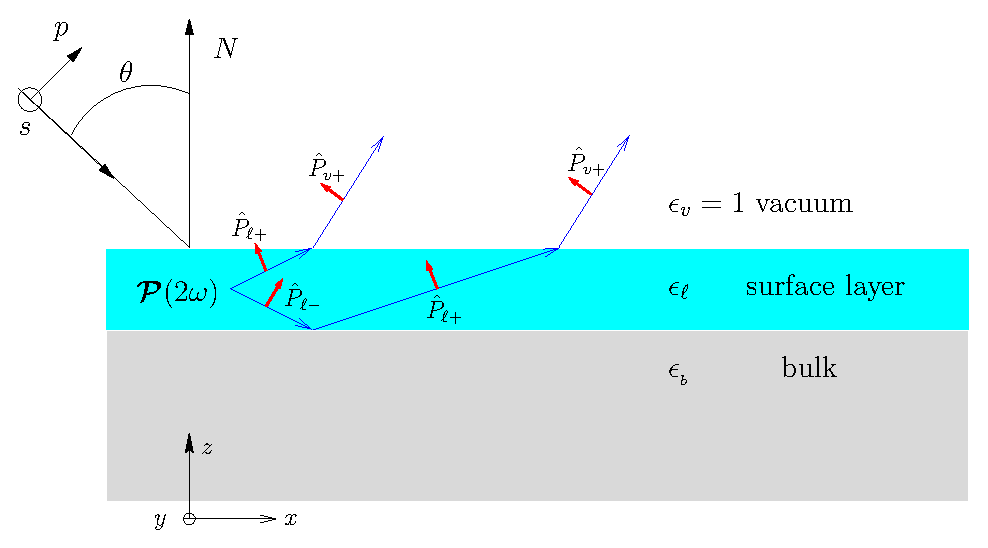
\includegraphics[scale=.5]{figures/3layers}
\caption{Sketch of the three layer model for SHG. Vacuum is on top with
$\epsilon=1$, the layer with nonlinear polarization $\mathbf{P}(2\omega)$
ischaracterized with $\epsilon_{\ell}(\omega)$ and the bulk with
$\epsilon_{b}(\omega)$. In the dipolar approximation the bulk does not radiate
SHG. The thin arrows are along the direction of propagation, and the unit
vectors for $p$-polarization are denoted with thick arrows (capital letters
denote SH components). The unit vector for $s$-polarization points along $-y$
(out of the page).}
\label{3layer}
\end{figure}

In the above equations $z$ is the direction perpendicular to the surface that
points towards the vacuum, $x$ is parallel to the surface, and $\theta$ is the
angle of incidence, where the plane of incidence is chosen as the $xz$ plane
(see Fig. \ref{3layer}), thus $\hat{\mathbf{s}}=-\hat{\mathbf{y}}$. The
function $k_i(\omega)$ is the projection of the wave vector perpendicular to
the surface. As we see from Fig. \ref{3layer}, the SH field is refracted at the
layer-vacuum interface ($\ell v$), and reflected from the layer-bulk ($\ell b$)
interface, thus we can define the transmission, $\mathbf{T}$, and reflection,
$\mathbf{R}$, tensors as,
\begin{equation*}\label{r5}
\mathbf{T}_{\ell v}
= \hat{\mathbf{s}}T_s^{\ell v}\hat{\mathbf{s}} 
+ \hat{\mathbf{P}}_{v+}T_{p}^{\ell v} \hat{\mathbf{P}}_{\ell +},
\end{equation*}
and
\begin{equation*}\label{r6}
\mathbf{R}_{\ell b}
= \hat{\mathbf{s}}R_s^{\ell b}\hat{\mathbf{s}}
+ \hat{\mathbf{P}}_{\ell +}R_{p}^{\ell b} \hat{\mathbf{P}}_{\ell -},
\end{equation*}
where variables in capital letters are evaluated at the harmonic frequency
$2\omega$. Notice that since $\hat{\mathbf{s}}$ is independent of $\omega$,
then $\hat{\mathbf{S}}=\hat{\mathbf{s}}$. The Fresnel factors, $T_i$, $R_i$,
for $i=s,p$ polarization, are evaluated at the appropriate interface $\ell v$
or $\ell b$, and will be given below. The extra subscript in $\hat{\mathbf{P}}$
denotes the corresponding dielectric function to be used in its evaluation,
i.e. $\epsilon_v=1$ for vacuum ($v$), $\epsilon_{\ell}$ for the layer ($\ell$),
and $\epsilon_{b}$ for the bulk ($b$). Therefore, the total radiated field at
$2\omega$ is
\begin{equation*}\label{r7}
\begin{split}
\mathbf{E}(2\omega)
&= E_s(2\omega)
\left(
\mathbf{T}^{\ell v} + \mathbf{T}^{\ell v}\cdot\mathbf{R}^{\ell b}
\right)
\cdot\hat{\mathbf{s}}\nonumber\\
&+ E_{p+}(2\omega)\mathbf{T}^{\ell v}\cdot\hat{\mathbf{P}}_{\ell +}
 + E_{p-}(2\omega)\mathbf{T}^{\ell v}
\cdot\mathbf{R}^{\ell b}\cdot\hat{\mathbf{P}}_{\ell-}.
\end{split}
\end{equation*}
The first term is  the transmitted $s$-polarized field, the second one is the
reflected and then transmitted $s$-polarized field and the third and fourth
terms are the equivalent fields for $p$-polarization. The transmission is from
the layer into vacuum, and the reflection between the layer and the bulk. After
some simple algebra, we obtain
\begin{equation*}\label{r8}
\mathbf{E}(2\omega) = \frac{2\pi i\tilde{\Omega}}{K_{\ell}}
\mathbf{H}_{\ell}\cdot\boldsymbol{\mathcal{P}}(2\omega),
\end{equation*}
where,
\begin{equation}\label{r9}
\mathbf{H}_{\ell}
= \hat{\mathbf{s}}\,T_s^{\ell v}\left(1+R_s^{\ell b}\right)\hat{\mathbf{s}}
+ \hat{\mathbf{P}}_{v+}T_{p}^{\ell v}
\left(
\hat{\mathbf{P}}_{\ell +} +R_{p}^{\ell b}\hat{\mathbf{P}}_{\ell -}
\right). 
\end{equation}
The magnitude of the radiated field is given by
$E(2\omega)=\hat{\mathbf{e}}^{\mathrm{out}}\cdot\mathbf{E}(2\omega)$, where
$\hat{\mathbf{e}}^{\mathrm{out}}$ is the polarization vector of the radiated
field, for instance $\hat{\mathbf{s}}$ or $\hat{\mathbf{P}}_{v+}$. Then, we
write
\begin{equation*}\label{m1}
\begin{split}
\hat{\mathbf{P}}_{\ell +} + R_{p}^{\ell b}\hat{\mathbf{P}}_{\ell -}
&= \frac{\sin\theta_{\mathrm{in}}\hat{\mathbf{z}} - K_{\ell}\hat{\mathbf{x}}}
        {\sqrt{\epsilon_{\ell}(2\omega)}}
 + R_{p}^{\ell b}
   \frac{\sin\theta_{\mathrm{in}}\hat{\mathbf{z}} + K_{\ell}\hat{\mathbf{x}}}
        {\sqrt{\epsilon_{\ell}(2\omega)}}
\\\nonumber
&= \frac{1}{\sqrt{\epsilon_{\ell}(2\omega)}}
\left(
\sin\theta_{\mathrm{in}}(1+R^{\ell b}_{p})\hat{\mathbf{z}}
- K_{\ell}(1-R^{\ell b}_{p})\hat{\mathbf{x}} 
\right)
\\\nonumber 
&= \frac{T^{\ell b}_{p}}{\epsilon_{\ell}(2\omega)\sqrt{\epsilon_{b}(2\omega)}}
\left(
  \epsilon_{b}(2\omega)\sin\theta_{\mathrm{in}}\hat{\mathbf{z}} 
- \epsilon_{\ell}(2\omega)K_{b}\hat{\mathbf{x}}
\right)
,
\end{split}
\end{equation*}
where using
\begin{align}
1 + R^{\ell b}_{s} &= T^{\ell b}_{s}\nonumber\\
1 + R^{\ell b}_{p}
&= \sqrt{\frac{\epsilon_{b}(2\omega)}{\epsilon_{\ell}(2\omega)}}T^{\ell b}_{p} 
\nonumber\\
1 - R^{\ell b}_{p}
&= \sqrt{\frac{\epsilon_{\ell}(2\omega)}{\epsilon_{b}(2\omega)}}
   \frac{K_{b}}{K_{\ell}}T^{\ell b}_{p}\\
T^{\ell v}_{p} &= \frac{K_{\ell}}{K_{v}}T^{v\ell}_{p}\nonumber\\
T^{\ell v}_{s} &= \frac{K_{\ell}}{K_{v}}T^{v\ell}_{s}\nonumber
,
\end{align}
we can write
\begin{equation*}\label{r10}
E(2\omega) = \frac{4\pi i \omega}{cK_{v}}
\hat{\mathbf{e}}^{\mathrm{out}}\cdot
\mathbf{H}_{\ell}\cdot
\boldsymbol{\mathcal{P}}(2\omega) 
= \frac{4\pi i\omega}{cK_{v}}
  \mathbf{e}^{\,2\omega}_{\ell}\cdot\boldsymbol{\mathcal{P}}(2\omega). 
\end{equation*}
where,
\begin{equation}\label{r12}
\begin{split}
\mathbf{e}^{2\omega}_{\ell} &= \\ &\hat{\mathbf{e}}^{\mathrm{out}}\cdot
\Bigg[
\hat{\mathbf{s}}T_{s}^{v\ell}T_{s}^{\ell b}\hat{\mathbf{s}} + 
\hat{\mathbf{P}}_{v+}
\frac{T^{v\ell}_{p}T^{\ell b}_{p}}
     {\epsilon_{\ell}({2\omega})\sqrt{\epsilon_{b}(2\omega)}}
\left(
  \epsilon_{b}(2\omega)\sin\theta_{\mathrm{in}}\hat{\mathbf{z}}
- \epsilon_{\ell}(2\omega)K_{b}\hat{\mathbf{x}}
\right)
\Bigg]
.
\end{split}
\end{equation}  
% We mention that
% $n_v\sin\theta_{\mathrm{in}}=n_{\ell}\sin\theta_{\mathrm{in}}$, from which
% $\sin\theta_{\mathrm{in}}=\sin\theta_{\mathrm{in}}/n_{\ell}$ with
% $n_i=\sqrt{\epsilon_i(\omega)}$.

We pause here to reduce above result to the case where the nonlinear
polarization $\mathbf{P}(2\omega)$ radiates from vacuum instead from the layer
$\ell$. For such case we simply take $\epsilon_{\ell}(2\omega)=1$ and $\ell=v$
($T^{\ell v}_{s,p}=1$), to get
\begin{equation}\label{r13}
\mathbf{e}^{\,2\omega}_{v} = \hat{\mathbf{e}}^{\mathrm{out}}
\cdot\left[
\hat{\mathbf{s}}T_s^{v b}\hat{\mathbf{s}} + \hat{\mathbf{P}}_{v+}
\frac{T^{v b}_{p}}{\sqrt{\epsilon_{b}(2\omega)}}
\left(
  \epsilon_{b}(2\omega)\sin\theta_{\mathrm{in}}\hat{\mathbf{z}}
  - K_{b}\hat{\mathbf{x}}
\right) 
\right] 
,
\end{equation}
which agrees with Eq. (3.8) of Ref. \cite{mizrahiJOSA88}.

In the three layer model the nonlinear polarization is located in layer $\ell$,
and then we evaluate the fundamental field required in Eq. \eqref{tres} in this
layer as well, then we write
\begin{equation}\label{m2}
\mathbf{E}_{\ell}(\omega)=E_0\left(
\hat{\mathbf{s}} t^{v\ell}_s(1+r^{\ell b}_s)\hat{\mathbf{s}}
+
\hat{\mathbf{p}}_{\ell-}
 t^{v\ell}_{p}
\hat{\mathbf{p}}_{v-}
+
\hat{\mathbf{p}}_{\ell+}
t^{v\ell}_{p}r^{\ell b}_{p}
\hat{\mathbf{p}}_{v-}
\right)\cdot\hat{\mathbf{e}}^{\mathrm{in}}=E_0\mathbf{e}^\omega_{\ell}
,
\end{equation} 
and following the steps that lead to Eq. \eqref{r12}, we find that
\begin{equation}\label{m12}
\mathbf{e}^{\omega}_{\ell}
= \left[
\hat{\mathbf{s}}t_{s}^{v\ell}t_{s}^{\ell b}\hat{\mathbf{s}} 
+ \frac{t^{v\ell}_{p}t^{\ell b}_{p}}
       {\epsilon_{\ell}(\omega)\sqrt{\epsilon_{b}(\omega)}}
\left(
  \epsilon_{b}(\omega)\sin\theta_{\mathrm{in}}\hat{\mathbf{z}}
+ \epsilon_{\ell}(\omega)k_{b}\hat{\mathbf{x}}
\right)
\hat{\mathbf{p}}_{v-}
\right]
\cdot\hat{\mathbf{e}}^{\mathrm{in}}.  
\end{equation}  
If we would like to evaluate the fields in the bulk, instead of the layer
$\ell$, we simply take $\epsilon_{\ell}(\omega)=\epsilon_{b}(\omega)\,(t^{\ell
b}_{s,p}=1$), to obtain
\begin{equation}\label{m13}
\mathbf{e}^{\omega}_{b}
= \left[
\hat{\mathbf{s}}t_{s}^{vb}\hat{\mathbf{s}}
+ \frac{t^{vb}_{p}}{\sqrt{\epsilon_{b}(\omega)}}
\left(
\sin\theta_{\mathrm{in}}\hat{\mathbf{z}} + k_{b}\hat{\mathbf{x}}
\right) 
\hat{\mathbf{p}}_{v-}
\right]
\cdot\hat{\mathbf{e}}^{\mathrm{in}},  
\end{equation} 
that is in agreement with Eq. (3.5) of Ref. \cite{mizrahiJOSA88}.

With $\mathbf{e}^{\omega}$ we can write Eq. \eqref{tres} as
\begin{equation*}\label{m4}
\boldsymbol{\mathcal{P}}(2\omega) = E^{2}_{0}\boldsymbol{\chi}:
\mathbf{e}^{\omega}_{\ell}\mathbf{e}^{\omega}_{\ell}
,
\end{equation*}
and then from Eq. \eqref{r10} we obtain that
\begin{align}\label{r01}
|E(2\omega)|^2 
&= |E_{0}|^4\frac{16\pi^{2}\omega^{2}}{c^{2}K^{2}_{v}}
\left\vert
\mathbf{e}^{\,2\omega}_{\ell}\cdot\boldsymbol{\chi}:
\mathbf{e}^{\omega}_{\ell}\mathbf{e}^{\omega}_{\ell}
\right\vert^{2}
\nonumber\\
\frac{c}{2\pi}|E(2\omega)|^{2} 
&= \frac{32\pi^{3}\omega^{2}}{c^{3}\cos^{2}\theta_{\mathrm{in}}}
\left\vert
\mathbf{e}^{\,2\omega}_{\ell}\cdot\boldsymbol{\chi}:
\mathbf{e}^{\omega}_{\ell}\mathbf{e}^{\omega}_{\ell}
\right\vert^{2} 
\left(\frac{c}{2\pi}|E_{0}|^{2}\right)^{2},
\nonumber\\
I(2\omega) 
&= \frac{32\pi^{3}\omega^{2}}{c^{3}\cos^{2}\theta_{\mathrm{in}}}
\left\vert
\mathbf{e}^{\,2\omega}_{\ell}\cdot\boldsymbol{\chi}:
\mathbf{e}^\omega_{\ell}\mathbf{e}^\omega_{\ell}
\right\vert^{2}I^{2}(\omega),
\nonumber\\
R(2\omega) 
&= \frac{32\pi^{3}\omega^{2}}{c^{3}\cos^{2}\theta_{\mathrm{in}}}
\left\vert
\mathbf{e}^{\,2\omega}_{\ell}\cdot\boldsymbol{\chi}:
\mathbf{e}^{\omega}_{\ell}\mathbf{e}^{\omega}_{\ell}\right\vert^{2} 
,
\end{align}
as the SHG yield. At this point we mention that to recover the results of Ref.
\cite{mizrahiJOSA88} which are equivalent of those of Ref. \cite{sipePRB87}, we
take $\mathbf{e}^{2\omega}_{\ell}\to \mathbf{e}^{2\omega}_v$,
$\mathbf{e}^{\omega}_{\ell}\to \mathbf{e}^{\omega}_{b}$ and then
\begin{equation}\label{m69}
R(2\omega) =
\frac{32\pi^{3} \omega^{2}}{c^{3}\cos^{2}\theta_{\mathrm{in}}}
\left\vert
\mathbf{e}^{\,2\omega}_{v}\cdot\boldsymbol{\chi}:
\mathbf{e}^{\omega}_{b}\mathbf{e}^{\omega}_{b}
\right\vert^{2} 
,
\end{equation}
will give the SHG yield of a nonlinear polarization sheet radiating from vacuum
on top of the surface and where the fundamental field is evaluated below the
surface that is characterized by $\epsilon_{b}(\omega)$.

To complete the required formulas, we write down the Fresnel factors,
\begin{equation*}\label{e.f1}
\begin{split}
t_s^{ij}(\omega) &=
\frac{2k_{i}(\omega)}{k_{i}(\omega)+k_{j}(\omega)},
\quad\quad  
t_{p}^{ij}(\omega) =
\frac{2k_{i}(\omega)\sqrt{\epsilon_{i}(\omega)\epsilon_j(\omega)}}
     {k_{i}(\omega)\epsilon_{j}(\omega)+k_{j}(\omega)\epsilon_{i}(\omega)},\\
r_s^{ij}(\omega) &=
\frac{k_{i}(\omega) - k_{j}(\omega)}
     {k_{i}(\omega) + k_{j}(\omega)},
\quad\quad 
r_{p}^{ij}(\omega) =
\frac{k_{i}(\omega)\epsilon_{j}(\omega) - k_{j}\epsilon_{i}(\omega)}
     {k_{i}(\omega)\epsilon_{j}(\omega) + k_{j}(\omega)\epsilon_{i}(\omega)}.
\end{split}
\end{equation*}


\section{\texorpdfstring{$\mathcal{R}$}{R} for different polarization cases}

We obtain explicit relations for a $C_{3v}$ symmetry characteristic of a (111)
surface, for which the only components of $\chi_{ijk}$ different from zero are
$\chi_{zzz}$, $\chi_{zxx}=\chi_{zyy}$, $\chi_{xxz}=\chi_{yyz}$ and
$\chi_{xxx}=-\chi_{xyy}=-\chi_{yyx}$ with $\chi_{ijk}=\chi_{ikj}$, where we
have chosen the $x$ and $y$ axes along the [112] and [110] directions,
respectively.

However, we have to remember that the plane of incidence so far was chosen to
be the $xz$ plane; the most general plane of incidence should be one that makes
an angle $\phi$ with respect to the $x$ axis, and so $\hat{\mathbf{x}}$ should
to be replaced by a unit vector $\hat{\mathbf{\kappa}}$ such that
\begin{equation}\label{mc1}
\hat{\boldsymbol{\kappa}}
= \cos\phi\hat{\mathbf{x}} + \sin\phi\hat{\mathbf{y}},
\end{equation}
and then
\begin{equation}\label{mc2}
\hat{\mathbf{s}} = -\sin\phi\hat{\mathbf{x}} + \cos\phi\hat{\mathbf{y}},
\end{equation}

\subsection{\texorpdfstring{$\mathcal{R}_{pP}$}{RpP}}

To obtain $R_{pP}(2\omega)$ we use
$\mathbf{e}^{\mathrm{in}}=\hat{\mathbf{p}}_{v-}$ in Eq. \eqref{m12}, and
$\mathbf{e}^{\mathrm{out}}=\hat{\mathbf{P}}_{v+}$ in Eq. \eqref{r12}, to obtain
that for a $C_{3v}$ symmetry characteristic of a (111) surface,
\begin{equation*}\label{m80}
\mathbf{e}^{\,2\omega}_{\ell}\cdot\boldsymbol{\chi}:
\mathbf{e}^\omega_{\ell}\mathbf{e}^\omega_{\ell}
\equiv\Gamma^{\ell}_{pP}\,r^{\ell}_{pP}
,
\end{equation*}
where
\begin{align}\label{m81}
r^{\ell}_{pP} &=
\epsilon_{b}(2\omega)\sin\theta_{\mathrm{in}}
\Big(
  \epsilon^2_{b}(\omega)\sin^2\theta_{\mathrm{in}}\chi_{zzz}
+ \epsilon^2_{\ell}(\omega)k^2_{b}\chi_{zxx}
\Big)\\
&- \epsilon_{\ell}(2\omega)\epsilon_{\ell}(\omega)k_{b}K_{b}
\Big(
  2\epsilon_{b}(\omega)\sin\theta_{\mathrm{in}}\chi_{xxz}
+ \epsilon_{\ell}(\omega)k_{b}\chi_{xxx}\cos(3\phi) 
\Big),\nonumber
\end{align}
and  
\begin{equation}\label{m79}
\Gamma^{\ell}_{pP}=
\frac{T_{p}^{\ell v}T^{\ell b}_{p}}
     {\epsilon_{\ell}(2\omega)\sqrt{\epsilon_{b}(2\omega)}}
\left(
\frac{t_{p}^{v\ell}t^{\ell b}_{p}}
     {\epsilon_{\ell}(\omega)\sqrt{\epsilon_{b}(\omega)}}
\right)^{2} 
.  
\end{equation} 
In order to reduce above result to that of Ref. \cite{mizrahiJOSA88} and
\cite{sipePRB87},  we take the $2\omega$ radiations factors for vacuum by
taking $\ell=v$, thus $\epsilon_{\ell}(2\omega)=1$, $T^{\ell v}_{p}=1$,
$T^{\ell b}_{p}=T^{vb}_{p}$, and the fundamental field inside medium $b$ by
taking $\ell=b$, thus $\epsilon_{\ell}(\omega)=\epsilon_{b}(\omega)$,
$t^{v\ell}_{p}=t^{vb}_{p}$, and $t^{\ell b}_{p}=1$. With these choices,
\begin{equation*}\label{m82}
\begin{split}
r^{b}_{pP}
&= \epsilon_{b}(2\omega)\sin\theta_{\mathrm{in}}
\Big(
\sin^2\theta_{\mathrm{in}}\chi_{zzz} + k^{2}_{b}chi_{zxx}
\Big)\\
&- k_{b}K_{b}
\Big(
2\sin\theta_{\mathrm{in}}\chi_{xxz} + k_{b}\chi_{xxx}\cos(3\phi) 
\Big) 
,
\end{split}
\end{equation*}
and 
\begin{equation*}\label{m78}
\Gamma^b_{pP}
= \frac{T^{v b}_{p}(t^{vb}_{p})^2}
       {\epsilon_{b}(\omega)\sqrt{\epsilon_{b}(2\omega)}}.
\end{equation*}


\subsubsection{Taking all fields in the bulk}
To evaluate the $2\omega$ fields in the bulk, we take Eq. \eqref{r9}
considering that $\ell\rightarrow b$. We have already considered the $1\omega$
fields in the bulk in Eq. \eqref{m13}. After some algebra, we get that
\begin{equation*}
\mathbf{e}^{\,2\omega}_{b}\cdot
\boldsymbol{\chi}:\mathbf{e}^{\omega}_{b}\mathbf{e}^{\omega}_{b} =
\Gamma^{b}_{pP}r^{b}_{pP}
\end{equation*}
where
\begin{equation*}
r^{b}_{pP} = 
  \sin^{3}\theta_{\mathrm{in}}\chi_{zzz} 
+ k^{2}_{b}\sin\theta_{\mathrm{in}}\chi_{zxx}
- 2k_{b}K_{b}\sin\theta_{\mathrm{in}}\chi_{xxz}
- k^{2}_{b}K_{b}\chi_{xxx}\cos3\phi,
\end{equation*}
and
\begin{equation*}
\Gamma^{b}_{pP} =
\frac{T_{p}^{vb}\left(t^{vb}_{p}\right)^{2}}
     {\epsilon_{b}(\omega)\sqrt{\epsilon_{b}(2\omega)}}.
\end{equation*}


\subsubsection{Taking all fields in the vacuum}
To evaluate the $1\omega$ fields in the vacuum, we take Eq. \eqref{m2}
considering that $\ell\rightarrow v$. We have already considered the $2\omega$
fields in the vacuum in Eq. \eqref{r13}. After some algebra, we get that
\begin{equation*}
\mathbf{e}^{\,2\omega}_{v}\cdot
\boldsymbol{\chi}:\mathbf{e}^{\omega}_{v}\mathbf{e}^{\omega}_{v} =
\Gamma^{v}_{pP}r^{v}_{pP}
\end{equation*}
where
\begin{equation*}
\begin{split}
r^{v}_{pP} &=
    \epsilon^{2}_{b}(\omega)\epsilon_{b}(2\omega)
    \sin^{3}\theta_{\mathrm{in}}\chi_{zzz}
 +  \epsilon_{b}(2\omega)k^{2}_{b}\sin\theta_{\mathrm{in}}\chi_{zxx}\\
&- 2\epsilon_{b}(\omega)k_{b}K_{b}\sin\theta_{\mathrm{in}}\chi_{xxz}
 -  k^{2}_{b}K_{b}\chi_{xxx}\cos3\phi
\end{split}
\end{equation*}
and
\begin{equation*}
\Gamma^{v}_{pP} =
\frac{T^{v b}_{p}\left(t^{v b}_{p}\right)^{2}}
     {\epsilon_{b}(\omega)\sqrt{\epsilon_{b}(2\omega)}}.
\end{equation*}


\subsection{\texorpdfstring{$\mathcal{R}_{pS}$}{RpS}}

To obtain $R_{pS}(2\omega)$ we use
$\mathbf{e}^{\mathrm{in}}=\hat{\mathbf{p}}_{v-}$ in Eq. \eqref{m12}, and
$\mathbf{e}^{\mathrm{out}}=\hat{\mathbf{S}}$ in Eq. \eqref{r12}. We also use
the unit vectors defined in Eqs. \eqref{mc1} and
\eqref{mc2}. Substituting, we get
\begin{equation*}
\mathbf{e}^{\,2\omega}_{\ell}\cdot
\boldsymbol{\chi}:\mathbf{e}^\omega_{\ell}\mathbf{e}^\omega_{\ell}
\equiv\Gamma^{\ell}_{sP}\, r^{\ell}_{sP},
\end{equation*}
where
\begin{equation}
r^{\ell}_{pS}
= -\epsilon^{2}_{\ell}(\omega)k^{2}_{b}\sin3\phi\chi_{xxx},
\end{equation} 
and  
\begin{equation}
\Gamma^{\ell}_{pS} =
T^{v\ell}_{s}T^{\ell b}_{s}\left(\frac{t^{v\ell}_{p}t^{\ell b}_{p}}
      {\epsilon_{\ell}(\omega)\sqrt{\epsilon_{b}(\omega)}}\right)^{2}.
\end{equation} 
In order to reduce above result to that of Ref. \cite{mizrahiJOSA88} and
\cite{sipePRB87},  we take the $2\omega$ radiations factors for vacuum by
taking $\ell=v$, thus $\epsilon_{\ell}(2\omega)=1$, $T^{v\ell}_{s}=1$,
$T^{\ell b}_{s}=T^{vb}_{s}$, and the fundamental field inside medium $b$ by
taking $\ell=b$, thus $\epsilon_{\ell}(\omega)=\epsilon_{b}(\omega)$,
$t^{v\ell}_{p}=t^{vb}_{p}$, and $t^{\ell b}_{p}=1$. With these choices,
\begin{equation*}
r^{b}_{pS} = -k^{2}_{b}\sin3\phi\chi_{xxx},
\end{equation*} 
and 
\begin{equation*}
\Gamma^{b}_{pS} =
T^{vb}_{s}
\left(
\frac{t^{vb}_{p}}{\sqrt{\epsilon_{b}(\omega)}}
\right)^{2}.  
\end{equation*} 


\subsection{\texorpdfstring{$\mathcal{R}_{sP}$}{RsP}}

To obtain $R_{sP}(2\omega)$ we use $\mathbf{e}^{\mathrm{in}}=\hat{\mathbf{s}}$
in Eq. \eqref{m12}, and $\mathbf{e}^{\mathrm{out}}=\hat{\mathbf{P}}_{v+}$ in
Eq. \eqref{r12}. We also use the unit vectors defined in Eqs. \eqref{mc1} and
\eqref{mc2}. Substituting, we get
\begin{equation*}
\mathbf{e}^{\,2\omega}_{\ell}\cdot
\boldsymbol{\chi}:\mathbf{e}^\omega_{\ell}\mathbf{e}^\omega_{\ell}
\equiv\Gamma^{\ell}_{sP}\, r^{\ell}_{sP},
\end{equation*}
where
\begin{equation}
r^{\ell}_{sP}
= \epsilon_{b}(2\omega)\sin\theta_{\mathrm{in}}\chi_{zxx}
+ \epsilon_{\ell}(2\omega)K_{b}\chi_{xxx}\cos3\phi,
\end{equation} 
and  
\begin{equation}
\Gamma^{\ell}_{sP}=
\frac{T_{p}^{\ell v}T^{\ell b}_{p}\left(t_s^{v\ell}t^{\ell b}_s\right)^2}
     {\epsilon_{\ell}(2\omega)\sqrt{\epsilon_{b}(2\omega)}}.  
\end{equation} 
In order to reduce above result to that of Ref. \cite{mizrahiJOSA88} and
\cite{sipePRB87}, we take the $2\omega$ radiations factors for vacuum by
taking $\ell=v$, thus $\epsilon_{\ell}(2\omega)=1$, $T^{v\ell}_{p}=1$,
$T^{\ell b}_{p}=T^{vb}_{p}$, and the fundamental field inside medium $b$ by
taking $\ell=b$, thus $\epsilon_{\ell}(\omega)=\epsilon_{b}(\omega)$,
$t^{v\ell}_s=t^{vb}_s$, and $t^{\ell b}_s=1$. With these choices,
\begin{equation*}
r^{b}_{sP} = \epsilon_{b}(2\omega)\sin\theta_{\mathrm{in}}\chi_{zxx}
+ K_{b}\chi_{xxx}\cos3\phi,
\end{equation*} 
and 
\begin{equation*}
\Gamma^{b}_{sP} =
\frac{T^{v b}_{p}(t_s^{vb})^{2}}{\sqrt{\epsilon_{b}(2\omega)}}.  
\end{equation*} 


\subsection{\texorpdfstring{$\mathcal{R}_{sS}$}{RsS}}

For $\mathcal{R}_{sS}$ we have that
$\mathbf{e}^{\mathrm{in}}=\hat{\mathbf{s}}$ and
$\mathbf{e}^{\mathrm{out}}=\hat{\mathbf{S}}$. This leads to
\begin{equation*}
\mathbf{e}^{\,2\omega}_{\ell}\cdot
\boldsymbol{\chi}:\mathbf{e}^\omega_{\ell}\mathbf{e}^\omega_{\ell}
\equiv\Gamma^{\ell}_{sS}\, r^{\ell}_{sS},
\end{equation*}
where
\begin{equation}
r^{\ell}_{sS} = \chi_{xxx}\sin3\phi,
\end{equation}
and
\begin{equation}
\Gamma^{\ell}_{sS}=
T^{v\ell}_{s}T^{\ell b}_{s}\left(t^{v\ell}_{s}t^{\ell b}_{s}\right)^{2}.
\end{equation} 
In order to reduce above result to that of Ref. \cite{mizrahiJOSA88} and
\cite{sipePRB87}, we take the $2\omega$ radiations factors for vacuum by
taking $\ell=v$, thus $\epsilon_{\ell}(2\omega)=1$, $T^{v\ell}_{s}=1$,
$T^{\ell b}_{s}=T^{vb}_{s}$, and the fundamental field inside medium $b$ by
taking $\ell=b$, thus $\epsilon_{\ell}(\omega)=\epsilon_{b}(\omega)$,
$t^{v\ell}_{s}=t^{vb}_{s}$, and $t^{\ell b}_{s}=1$. With these choices,
\begin{equation*}
r^{b}_{sS} = \chi_{xxx}\sin3\phi,
\end{equation*}
and 
\begin{equation*}
\Gamma^{b}_{sS} = T^{vb}_{s}\left(t^{vb}_{s}\right)^{2}.
\end{equation*} 


\appendix
\chapter{Derived expressions for the SHG yield}
%%%%%%%%%%%%%%%%%%%%%%%%%%%%%%%%%%%%%%%%%%%%%%%%%%%%%%%%%%%%%%%%%%%%%%%%%%%%%%%%
%%%%%%%%%%%%%%%%%%%%%%%%%%%%%%%%%%%%%%%%%%%%%%%%%%%%%%%%%%%%%%%%%%%%%%%%%%%%%%%%


\section{Some useful expressions}
We are interested in finding
\begin{equation*}
\Upsilon = 
\mathbf{e}^{2\omega}_{\ell}\cdot\boldsymbol{\chi}:
\mathbf{e}^{\omega}_{\ell}\mathbf{e}^{\omega}_{\ell}
\end{equation*}
for each different polarization case. We choose the plane of incidence
along the $\boldsymbol{\kappa}z$ plane, and define 
\begin{equation}\label{eq:kappavec}
\hat{\boldsymbol{\kappa}}
= \cos\phi\hat{\mathbf{x}} + \sin\phi\hat{\mathbf{y}},
\end{equation}
and
\begin{equation}\label{eq:svec}
\hat{\mathbf{s}} = -\sin\phi\hat{\mathbf{x}} + \cos\phi\hat{\mathbf{y}},
\end{equation}
where $\phi$ the angle with respect to the $x$ axis.


\subsection{\texorpdfstring{$2\omega$}{2w} terms}

Including multiple reflecions, the $\mathbf{e}^{2\omega}_{\ell}$ term is
\begin{equation}\label{eq:e2wellmr}
\mathbf{e}^{2\omega}_{\ell} = \hat{\mathbf{e}}^{\mathrm{out}}\cdot
\Bigg[
\hat{\mathbf{s}}T_{s}^{v\ell}R^{M+}_{s}\hat{\mathbf{s}} + 
\hat{\mathbf{P}}_{v+}\frac{T^{v\ell}_{p}}{N_{\ell}}
\left(
\sin\theta_{0}R^{M+}_{p}\hat{\mathbf{z}} 
- W_{\ell}R^{M-}_{p}\hat{\boldsymbol{\kappa}}
\right)
\Bigg],
\end{equation}
and neglecting the multiple reflections reduces this expression to
\begin{equation}\label{eq:e2well}
\begin{split}
\mathbf{e}^{2\omega}_{\ell} = 
\hat{\mathbf{e}}^{\mathrm{out}}\cdot
\Bigg[
\hat{\mathbf{s}}T_{s}^{v\ell}T_{s}^{\ell b}\hat{\mathbf{s}} + 
\hat{\mathbf{P}}_{v+}
\frac{T^{v\ell}_{p}T^{\ell b}_{p}}
     {N^{2}_{\ell}N_{b}}
\left(
N^{2}_{b}\sin\theta_{0}\hat{\mathbf{z}} - N^{2}_{\ell}W_{b}\hat{\mathbf{x}}
\right)
\Bigg].
\end{split}
\end{equation}  

We first expand these equations for clarity. Substituting Eqs.
\eqref{eq:kappavec} and \eqref{eq:svec} into Eq. \eqref{eq:e2wellmr},
\begin{equation*}\label{eq:e2wexpmr}
\begin{split}
\mathbf{e}^{2\omega}_{\ell} = \hat{\mathbf{e}}^{\mathrm{out}}&\cdot
\Bigg[
\hat{\mathbf{s}}T_{s}^{v\ell}R^{M+}_{s}
\left(
- \sin\phi\hat{\mathbf{x}}
+ \cos\phi\hat{\mathbf{y}}
\right)\\
&+ \hat{\mathbf{P}}_{v+}\frac{T^{v\ell}_{p}}{N_{\ell}}
\left(
  \sin\theta_{0}R^{M+}_{p}\hat{\mathbf{z}}
- W_{\ell}R^{M-}_{p}\cos\phi\hat{\mathbf{x}}
- W_{\ell}R^{M-}_{p}\sin\phi\hat{\mathbf{y}}
\right)
\Bigg].
\end{split}
\end{equation*}
We now have $\mathbf{e}^{2\omega}_{\ell}$ in terms of
$\hat{\mathbf{P}}_{v+}$,
\begin{equation}\label{eq:e2wpmr}
\mathbf{e}^{2\omega}_{\ell} =
\frac{T^{v\ell}_{p}}{N_{\ell}}
\left(
  \sin\theta_{0}R^{M+}_{p}\hat{\mathbf{z}}
- W_{\ell}R^{M-}_{p}\cos\phi\hat{\mathbf{x}}
- W_{\ell}R^{M-}_{p}\sin\phi\hat{\mathbf{y}}
\right),
\end{equation}
and in terms of $\hat{\mathbf{s}}$,
\begin{equation}\label{eq:e2wsmr}
\mathbf{e}^{2\omega}_{\ell} =
T_{s}^{v\ell}R^{M+}_{s}
\left(
- \sin\phi\hat{\mathbf{x}}
+ \cos\phi\hat{\mathbf{y}}
\right).
\end{equation}
Likewise, we do the exact same for Eq. \eqref{eq:e2well}, and get the
following term for $\hat{\mathbf{P}}_{v+}$,
\begin{equation}\label{eq:e2wp}
\mathbf{e}^{2\omega}_{\ell} =
\frac{T^{v\ell}_{p}T^{\ell b}_{p}}
     {N^{2}_{\ell}N_{b}}
\left(
  N^{2}_{b}\sin\theta_{0}\hat{\mathbf{z}}
- N^{2}_{\ell}W_{b}\cos\phi\hat{\mathbf{x}}
- N^{2}_{\ell}W_{b}\sin\phi\hat{\mathbf{y}}
\right),
\end{equation}
and $\hat{\mathbf{s}}$,
\begin{equation}\label{eq:e2ws}
\mathbf{e}^{2\omega}_{\ell} 
= T^{v\ell}_{s}T^{\ell b}_{s}
\left[-\sin\phi\hat{\mathbf{x}} + \cos\phi\hat{\mathbf{y}}\right].
\end{equation}


\subsection{\texorpdfstring{$1\omega$}{1w} terms}

We posit that the effects of the multiple reflections can be neglected for the
$\mathbf{e}^{\omega}_{\ell}$ term. This term is
\begin{equation*}\label{eq:ewell}
\mathbf{e}^{\omega}_{\ell} = 
\left[
\hat{\mathbf{s}}t_{s}^{v\ell}t_{s}^{\ell b}\hat{\mathbf{s}} 
+ \frac{t^{v\ell}_{p}t^{\ell b}_{p}}{n^{2}_{\ell}n_{b}}
\left(
  n^{2}_{b}\sin\theta_{0}\hat{\mathbf{z}} 
+ n^{2}_{\ell}w_{b}\hat{\boldsymbol{\kappa}}
\right)
\hat{\mathbf{p}}_{v-}
\right]
\cdot\hat{\mathbf{e}}^{\mathrm{in}}.
\end{equation*}
For all cases, we require a
$\mathbf{e}^{\omega}_{\ell}\mathbf{e}^{\omega}_{\ell}$ product. For brevity, we
will directly list these terms for both polarizations. For
$\hat{\mathbf{e}}^{\mathrm{in}} = \hat{\mathbf{p}}_{v-}$,
\begin{equation}\label{eq:ewewp}
\begin{split}
\mathbf{e}^{\omega}_{\ell}\mathbf{e}^{\omega}_{\ell}
= \left(\frac{t^{v\ell}_{p}t^{\ell b}_{p}}
{n^{2}_{\ell}n_{b}}\right)^{2}
\big(
  &n^{4}_{\ell}w^{2}_{b}\cos^{2}\phi
\hat{\mathbf{x}}\hat{\mathbf{x}}
+ 2n^{4}_{\ell}w^{2}_{b}\sin\phi\cos\phi
\hat{\mathbf{x}}\hat{\mathbf{y}}\\
&+ 2n^{2}_{\ell}n^{2}_{b}w_{b}\sin\theta_{0}\cos\phi
\hat{\mathbf{x}}\hat{\mathbf{z}}
+ n^{4}_{\ell}w^{2}_{b}\sin^{2}\phi
\hat{\mathbf{y}}\hat{\mathbf{y}}\\
&+ 2n^{2}_{\ell}n^{2}_{b}w_{b}\sin\theta_{0}\sin\phi
\hat{\mathbf{y}}\hat{\mathbf{z}}
+ n^{4}_{b}\sin^{2}\theta_{0}
\hat{\mathbf{z}}\hat{\mathbf{z}}
\big),
\end{split}
\end{equation}
and for $\hat{\mathbf{e}}^{\mathrm{in}} = \hat{\mathbf{s}}$,
\begin{equation}\label{eq:ewews}
\mathbf{e}^{\omega}_{\ell}\mathbf{e}^{\omega}_{\ell}
= \left(t^{v\ell}_{s}t^{\ell b}_{s}\right)^{2}
\left(
  \sin^{2}\phi\hat{\mathbf{x}}\hat{\mathbf{x}}
+ \cos^{2}\phi\hat{\mathbf{y}}\hat{\mathbf{y}} 
- 2\sin\phi\cos\phi\hat{\mathbf{x}}\hat{\mathbf{y}}
\right).
\end{equation}

We summarize these expressions in Table \ref{tab:review}. In order to derive the
equations for a given polarization case, we refer to the equations listed there.
Then it is simply a matter of multiplying the terms correctly and obtaining the
appropriate components of $\boldsymbol{\chi}(-2\omega; \omega, \omega)$.

\begin{table}[b]
\centering
\begin{tabular}{ | c l l | c | c | }
\hline
Case               & $\hat{\mathbf{e}}^{\mathrm{out}}$
                   & $\hat{\mathbf{e}}^{\mathrm{in}}$
                   & $\mathbf{e}^{2\omega}_{\ell}$
                   & $\mathbf{e}^{\omega}_{\ell}\mathbf{e}^{\omega}_{\ell}$ \\
\hline
$\mathcal{R}_{pP}$ & $\hat{\mathbf{P}}_{v+}$
                   & $\hat{\mathbf{p}}_{v-}$
                   &  Eq. \eqref{eq:e2wpmr} or \eqref{eq:e2wp}
                   & Eq. \eqref{eq:ewewp} \\
$\mathcal{R}_{pS}$ & $\hat{\mathbf{s}}$
                   & $\hat{\mathbf{p}}_{v-}$
                   &  Eq. \eqref{eq:e2wsmr} or \eqref{eq:e2ws}
                   & Eq. \eqref{eq:ewewp} \\
$\mathcal{R}_{sP}$ & $\hat{\mathbf{P}}_{v+}$
                   & $\hat{\mathbf{s}}$
                   &  Eq. \eqref{eq:e2wpmr} or \eqref{eq:e2wp}
                   & Eq. \eqref{eq:ewews} \\
$\mathcal{R}_{sS}$ & $\hat{\mathbf{s}}$
                   & $\hat{\mathbf{s}}$
                   &  Eq. \eqref{eq:e2wsmr} or \eqref{eq:e2ws}
                   & Eq. \eqref{eq:ewews} \\
\hline
\end{tabular}
\caption{Polarization unit vectors for $\hat{\mathbf{e}}^{\mathrm{out}}$ and
$\hat{\mathbf{e}}^{\mathrm{in}}$, and equations describing
$\mathbf{e}^{2\omega}_{\ell}$ and
$\mathbf{e}^{\omega}_{\ell}\mathbf{e}^{\omega}_{\ell}$ for each polarization
case. When there are two equations to choose from, the former includes the
effects of multiple reflections, and the latter neglects
them.\label{tab:review}}
\end{table}


\subsection{Nonzero components of \texorpdfstring{$\boldsymbol{\chi}(-2\omega;
\omega, \omega)$}{X(2w;-w,w)}}

For a (111) surface with $C_{3v}$ symmetry, we have the following nonzero
components: 
\begin{equation}\label{eq:nonzero111}
\begin{split}
\chi_{xxx}&=-\chi_{xyy}=-\chi_{yyx},\\
\chi_{xxz}&=\chi_{yyz},\\
\chi_{zxx}&=\chi_{zyy},\\
\chi_{zzz}&.
\end{split}
\end{equation}

For a (110) surface with $C_{2v}$ symmetry, we have the following nonzero
components: 
\begin{equation}\label{eq:nonzero110}
\chi_{xxz}, \chi_{yyz}, \chi_{zxx}, \chi_{zyy}, \chi_{zzz}.
\end{equation}

Lastly, for a (001) surface with $C_{4v}$ symmetry, we have the following
nonzero components:
\begin{equation}\label{eq:nonzero001}
\begin{split}
\chi_{xxz}&=\chi_{yyz},\\
\chi_{zxx}&=\chi_{zyy},\\
\chi_{zzz}&.
\end{split}
\end{equation}

%%%%%%%%%%%%%%%%%%%%%%%%%%%%%%%%%%%%%%%%%%%%%%%%%%%%%%%%%%%%%%%%%%%%%%%%%%%%%%%%
%%%%%%%%%%%%%%%%%%%%%%%%%%%%%%%%%%%%%%%%%%%%%%%%%%%%%%%%%%%%%%%%%%%%%%%%%%%%%%%%


\section{\texorpdfstring{$\mathcal{R}_{pP}$}{RpP}}

Per Table \ref{tab:review}, $\mathcal{R}_{pP}$ requires Eqs. \eqref{eq:e2wp}
and \eqref{eq:ewewp}. After some algebra, we obtain that
\begin{equation}\label{eq:rppfullmr}
\begin{split}
\Upsilon^{\mathrm{MR}}_{pP} =
\Gamma^{\mathrm{MR}}_{pP}
\bigg[
- R^{M-}_{p}&W_{\ell}\big(
   n^{4}_{\ell}w^{2}_{b}\cos^{3}\phi\chi_{xxx}
 + 2n^{4}_{\ell}w^{2}_{b}\sin\phi\cos^{2}\phi\chi_{xxy}\\
&+ 2n^{2}_{\ell}n^{2}_{b}w_{b}\sin\theta_{0}\cos^{2}\phi\chi_{xxz}
 + n^{4}_{\ell}w^{2}_{b}\sin^{2}\phi\cos\phi\chi_{xyy}\\
&+ 2n^{2}_{\ell}n^{2}_{b}w_{b}\sin\theta_{0}\sin\phi\cos\phi\chi_{xyz}
 + n^{4}_{b}\sin^{2}\theta_{0}\cos\phi\chi_{xzz}
 \big)\\\\
%%%%%%%%%%%%%%%%%%%%%%%%%%%%%%%%%%%%%%%%%%%%%%%%%%%%%%%%%%%%%
- R^{M-}_{p}&W_{\ell}\big(
  n^{4}_{\ell}w^{2}_{b}\sin\phi\cos^{2}\phi\chi_{yxx}
+ 2n^{4}_{\ell}w^{2}_{b}\sin^{2}\phi\cos\phi\chi_{yxy}\\
&+ 2n^{2}_{\ell}n^{2}_{b}w_{b}\sin\theta_{0}\sin\phi\cos\phi\chi_{yxz}
 + n^{4}_{\ell}w^{2}_{b}\sin^{3}\phi\chi_{yyy}\\
&+ 2n^{2}_{\ell}n^{2}_{b}w_{b}\sin\theta_{0}\sin^{2}\phi\chi_{yyz}
 + n^{4}_{b}\sin^{2}\theta_{0}\sin\phi\chi_{yzz}
 \big)\\\\
%%%%%%%%%%%%%%%%%%%%%%%%%%%%%%%%%%%%%%%%%%%%%%%%%%%%%%%%%%%%%
+ R^{M+}_{p}&\sin\theta_{0}\big(
  n^{4}_{\ell}w^{2}_{b}\cos^{2}\phi\chi_{zxx}
 + 2n^{4}_{\ell}w^{2}_{b}\sin\phi\cos\phi\chi_{zxy}\\
&+ n^{4}_{\ell}w^{2}_{b}\sin^{2}\phi\chi_{zyy}
 + 2n^{2}_{\ell}n^{2}_{b}w_{b}\sin\theta_{0}\cos\phi\chi_{zzx}\\
&+ 2n^{2}_{\ell}n^{2}_{b}w_{b}\sin\theta_{0}\sin\phi\chi_{zzy}
 + n^{4}_{b}\sin^{2}\theta_{0}\chi_{zzz}
 \big)
\bigg].
\end{split}
\end{equation}
We take this opportunity to introduce a quantity that will be repeated
throughout this section,
\begin{equation}\label{eq:gammappmr}
\Gamma^{\mathrm{MR}}_{pP} =
\frac{T^{v\ell}_{p}}{N_{\ell}}
\left(\frac{t^{v\ell}_{p}t^{\ell b}_{p}}
{n^{2}_{\ell}n_{b}}\right)^{2}.
\end{equation}

If we neglect the multiple reflections, as described in the manuscript, we have
that
\begin{equation}\label{eq:rppfull}
\begin{split}
\Upsilon_{pP} =
\Gamma_{pP}
%%%%%%%%%%%%%%%%%%%%%%%%%%%%%%%%%%%%%%%%%%%%
\bigg[
- N^{2}_{\ell}W_{b}\big(
&+ n^{4}_{\ell}w^{2}_{b}\cos^{3}\phi\chi_{xxx}
 + 2n^{4}_{\ell}w^{2}_{b}\sin\phi\cos^{2}\phi\chi_{xxy}\\
&+ 2n^{2}_{b}n^{2}_{\ell}w_{b}\sin\theta_{0}\cos^{2}\phi\chi_{xxz}
 + n^{4}_{\ell}w^{2}_{b}\sin^{2}\phi\cos\phi\chi_{xyy}\\
&+ 2n^{2}_{b}n^{2}_{\ell}w_{b}\sin\theta_{0}\sin\phi\cos\phi\chi_{xyz}
 + n^{4}_{b}\sin^{2}\theta_{0}\cos\phi\chi_{xzz}
  \big)\\\\
%%%%%%%%%%%%%%%%%%%%%%%%%%%%%
- N^{2}_{\ell}W_{b}\big(
&+ n^{4}_{\ell}w^{2}_{b}\sin\phi\cos^{2}\phi\chi_{yxx}
 + 2n^{4}_{\ell}w^{2}_{b}\sin^{2}\phi\cos\phi\chi_{yxy}\\
&+ 2n^{2}_{b}n^{2}_{\ell}w_{b}\sin\theta_{0}\sin\phi\cos\phi\chi_{yxz}
 + n^{4}_{\ell}w^{2}_{b}\sin^{3}\phi\chi_{yyy}\\
&+ 2n^{2}_{b}n^{2}_{\ell}w_{b}\sin\theta_{0}\sin^{2}\phi\chi_{yyz}
 + n^{4}_{b}\sin^{2}\theta_{0}\sin\phi\chi_{yzz}
  \big)\\\\
%%%%%%%%%%%%%%%%%%%%%%%%%%%%%%
+ N^{2}_{b}\sin\theta_{0}\big(
&+ n^{4}_{\ell}w^{2}_{b}\cos^{2}\phi\chi_{zxx}
 + 2n^{4}_{\ell}w^{2}_{b}\sin\phi\cos\phi\chi_{zxy}\\
&+ n^{4}_{\ell}w^{2}_{b}\sin^{2}\phi\chi_{zyy}
 + 2n^{2}_{\ell}n^{2}_{b}w_{b}\sin\theta_{0}\cos\phi\chi_{zzx}\\
&+ 2n^{2}_{\ell}n^{2}_{b}w_{b}\sin\theta_{0}\sin\phi\chi_{zzy}
 + n^{4}_{b}\sin^{2}\theta_{0}\chi_{zzz}
  \big)
\bigg],
\end{split}
\end{equation}
and again we introduce a quantity that will be repeated throughout this section,
\begin{equation}\label{gammapp}
\Gamma_{pP} =
\frac{T^{v\ell}_{p}T^{\ell b}_{p}}
     {N^{2}_{\ell}N_{b}}
\left(\frac{t^{v\ell}_{p}t^{\ell b}_{p}}
{n^{2}_{\ell}n_{b}}\right)^{2}.
\end{equation}


\subsection{For the (111) surface}

We take Eqs. \eqref{eq:rppfullmr} and \eqref{eq:nonzero111}, eliminate the
components that do not contribute, and apply the the symmetry relations as
follows,
\begin{equation*}
\begin{split}
\Upsilon^{\mathrm{MR},(111)}_{pP} =
\Gamma^{\mathrm{MR}}_{pP}
\big[
&+ R^{M+}_{p}n^{4}_{b}\sin^{3}\theta_{0}\chi_{zzz}\\
&+ R^{M+}_{p}n^{4}_{\ell}w^{2}_{b}\sin\theta_{0}\cos^{2}\phi\chi_{zxx}\\
&+ R^{M+}_{p}n^{4}_{\ell}w^{2}_{b}\sin\theta_{0}\sin^{2}\phi\chi_{zxx}\\
&- 2R^{M-}_{p}n^{2}_{\ell}n^{2}_{b}w_{b}W_{\ell}\sin\theta_{0}\cos^{2}\phi
   \chi_{xxz}\\
&- 2R^{M-}_{p}n^{2}_{\ell}n^{2}_{b}w_{b}W_{\ell}\sin\theta_{0}\sin^{2}\phi
   \chi_{xxz}\\
&- R^{M-}_{p}n^{4}_{\ell}w^{2}_{b}W_{\ell}\cos^{3}\phi\chi_{xxx}\\
&+ R^{M-}_{p}n^{4}_{\ell}w^{2}_{b}W_{\ell}\sin^{2}\phi\cos\phi\chi_{xxx}\\
&+ 2R^{M-}_{p}n^{4}_{\ell}w^{2}_{b}W_{\ell}\sin^{2}\phi\cos\phi\chi_{xxx}
\big].
\end{split}
\end{equation*}
We reduce terms,
\begin{equation*}
\begin{split}
\Upsilon^{\mathrm{MR},(111)}_{pP} &=
\Gamma^{\mathrm{MR}}_{pP}
\big[
+ R^{M+}_{p}n^{4}_{b}\sin^{3}\theta_{0}\chi_{zzz}\\
&\qquad\qquad+ R^{M+}_{p}n^{4}_{\ell}w^{2}_{b}\sin\theta_{0}
   (\sin^{2}\phi+\cos^{2}\phi)\chi_{zxx}\\
&\qquad\qquad- 2R^{M-}_{p}n^{2}_{\ell}n^{2}_{b}w_{b}W_{\ell}\sin\theta_{0}
   (\sin^{2}\phi+\cos^{2}\phi)\chi_{xxz}\\
&\qquad\qquad+ R^{M-}_{p}n^{4}_{\ell}w^{2}_{b}W_{\ell}
   (3\sin^{2}\phi\cos\phi - \cos^{3}\phi)\chi_{xxx}
\big]\\\\
&=
\Gamma^{\mathrm{MR}}_{pP}
\big[
R^{M+}_{p}\sin\theta_{0}(n^{4}_{b}\sin^{2}\theta_{0}\chi_{zzz} 
+ n^{4}_{\ell}w^{2}_{b}\chi_{zxx})\\
&\qquad\qquad- R^{M-}_{p}n^{2}_{\ell}w_{b}W_{\ell}(2n^{2}_{b}\sin\theta_{0}
\chi_{xxz}
+ n^{2}_{\ell}w_{b}\chi_{xxx}\cos3\phi)
\big]\\\\
& = \Gamma^{\mathrm{MR}}_{pP}\,r^{\mathrm{MR},(111)}_{pP},
\end{split}
\end{equation*}
where
\begin{equation}\label{eq:final-rpp.mr.111}
\begin{split}
r^{\mathrm{MR},(111)}_{pP} = 
&R^{M+}_{p}\sin\theta_{0}(n^{4}_{b}\sin^{2}\theta_{0}\chi_{zzz} 
+ n^{4}_{\ell}w^{2}_{b}\chi_{zxx})\\
&- R^{M-}_{p}n^{2}_{\ell}w_{b}W_{\ell}(2n^{2}_{b}\sin\theta_{0}\chi_{xxz}
+ n^{2}_{\ell}w_{b}\chi_{xxx}\cos3\phi).
\end{split}
\end{equation}

If we wish to neglect the effects of the multiple reflections, we follow the
exact same procedure but starting with Eq. \eqref{eq:rppfull},
\begin{equation*}
\begin{split}
\Upsilon^{(111)}_{pP}
= \Gamma_{pP}
\big[
&+ n^{4}_{b}N^{2}_{b}\sin^{3}\theta_{0}\chi_{zzz}\\
&+ n^{4}_{\ell}N^{2}_{b}w^{2}_{b}\sin\theta_{0}\cos^{2}\phi\chi_{zxx}\\
&+ n^{4}_{\ell}N^{2}_{b}w^{2}_{b}\sin\theta_{0}\sin^{2}\phi\chi_{zxx}\\
&- 2n^{2}_{b}n^{2}_{\ell}N^{2}_{\ell}w_{b}W_{b}\sin\theta_{0}\cos^{2}\phi
  \chi_{xxz}\\
&- 2n^{2}_{b}n^{2}_{\ell}N^{2}_{\ell}w_{b}W_{b}\sin\theta_{0}\sin^{2}\phi
  \chi_{xxz}\\
&- n^{4}_{\ell}N^{2}_{\ell}w^{2}_{b}W_{b}\cos^{3}\phi\chi_{xxx}\\
&+ n^{4}_{\ell}N^{2}_{\ell}w^{2}_{b}W_{b}\sin^{2}\phi\cos\phi\chi_{xxx}\\
&+ 2n^{4}_{\ell}N^{2}_{\ell}w^{2}_{b}W_{b}\sin^{2}\phi\cos\phi\chi_{xxx}
\big],
\end{split}
\end{equation*}
and reduce,
\begin{equation*}
\begin{split}
\Upsilon^{(111)}_{pP} &=
\Gamma_{pP}
\big[
+ n^{4}_{b}N^{2}_{b}
   \sin^{3}\theta_{0}\chi_{zzz}\\
&\qquad\qquad+ n^{4}_{\ell}N^{2}_{b}w^{2}_{b}
   \sin\theta_{0}(\sin^{2}\phi + \cos^{2}\phi)\chi_{zxx}\\
&\qquad\qquad- 2n^{2}_{b}n^{2}_{\ell}N^{2}_{\ell}w_{b}W_{b}
   \sin\theta_{0}(\sin^{2}\phi + \cos^{2}\phi)\phi\chi_{xxz}\\
&\qquad\qquad+ n^{4}_{\ell}N^{2}_{\ell}w^{2}_{b}W_{b}
   (3\sin^{2}\phi\cos\phi - \cos^{3}\phi)\chi_{xxx}
\big]\\\\
&=
\Gamma_{pP}
\big[
N^{2}_{b}\sin\theta_{0}(n^{4}_{b}\sin^{2}\theta_{0}\chi_{zzz} 
+ n^{4}_{\ell}w^{2}_{b}\chi_{zxx})\\
&\qquad\qquad- n^{2}_{\ell}N^{2}_{\ell}w_{b}W_{b}(2n^{2}_{b}\sin\theta_{0}
\chi_{xxz} 
 + n^{2}_{\ell}w_{b}\chi_{xxx}\cos3\phi)
\big]\\\\
&= \Gamma_{pP}\,r^{(111)}_{pP},
\end{split}
\end{equation*}
where
\begin{equation}\label{eq:final-rpp.111}
\begin{split}
r^{(111)}_{pP} = 
&N^{2}_{b}\sin\theta_{0}(n^{4}_{b}\sin^{2}\theta_{0}\chi_{zzz} 
+ n^{4}_{\ell}w^{2}_{b}\chi_{zxx})\\
&- n^{2}_{\ell}N^{2}_{\ell}w_{b}W_{b}(2n^{2}_{b}\sin\theta_{0}\chi_{xxz}
 + n^{2}_{\ell}w_{b}\chi_{xxx}\cos3\phi).
\end{split}
\end{equation}


\subsection{For the (110) surface}

We take Eqs. \eqref{eq:rppfullmr} and \eqref{eq:nonzero110}, eliminate the
components that do not contribute, and apply the the symmetry relations as
follows,
\begin{equation*}
\begin{split}
\Upsilon^{\mathrm{MR},(110)}_{pP} &=
\Gamma^{\mathrm{MR}}_{pP}
\bigg[
R^{M+}_{p}\sin\theta_{0}
\big(
  n^{4}_{b}\sin^{2}\theta_{0}\chi_{zzz}
+ n^{4}_{\ell}w^{2}_{b}(\sin^{2}\phi\chi_{zyy} + \cos^{2}\phi\chi_{zxx})
\big)\\
&\qquad- 2R^{M-}_{p}n^{2}_{\ell}n^{2}_{b}w_{b}W_{\ell}\sin\theta_{0}
(\sin^{2}\phi\chi_{yyz} + \cos^{2}\phi\chi_{xxz})
\bigg]\\\\
&=
\Gamma^{\mathrm{MR}}_{pP}
\bigg[
R^{M+}_{p}\sin\theta_{0}
\bigg(
  n^{4}_{b}\sin^{2}\theta_{0}\chi_{zzz}\\
&+ n^{4}_{\ell}w^{2}_{b}
\left(
\frac{1}{2}(1-\cos2\phi)\chi_{zyy} + \frac{1}{2}(\cos2\phi+1)\chi_{zxx}
\right)
\bigg)\\
&- 2R^{M-}_{p}n^{2}_{\ell}n^{2}_{b}w_{b}W_{\ell}\sin\theta_{0}
\left(
\frac{1}{2}(1-\cos2\phi)\chi_{yyz} + \frac{1}{2}(\cos2\phi+1)\chi_{xxz}
\right)
\bigg]\\\\
&=
\Gamma^{\mathrm{MR}}_{pP}
\bigg[
R^{M+}_{p}\sin\theta_{0}
\bigg(
n^{4}_{b}\sin^{2}\theta_{0}\chi_{zzz}\\
&\qquad+ n^{4}_{\ell}w^{2}_{b}
\left(
\frac{\chi_{zyy} + \chi_{zxx}}{2} + \frac{\chi_{zyy} - \chi_{zxx}}{2}\cos2\phi
\right)
\bigg)\\
&\qquad- 2R^{M-}_{p}n^{2}_{\ell}n^{2}_{b}w_{b}W_{\ell}\sin\theta_{0}
\left(
\frac{\chi_{yyz} + \chi_{xxz}}{2} + \frac{\chi_{yyz} - \chi_{xxz}}{2}\cos2\phi
\right)
\bigg]\\\\
&= \Gamma^{\mathrm{MR}}_{pP}\,r^{\mathrm{MR},(110)}_{pP},
\end{split}
\end{equation*}
where
\begin{equation}\label{eq:final-rpp.mr.110}
\begin{split}
r^{\mathrm{MR},(110)}_{pP} &= 
R^{M+}_{p}\sin\theta_{0}
\bigg[
n^{4}_{b}\sin^{2}\theta_{0}\chi_{zzz}\\
&\qquad+ n^{4}_{\ell}w^{2}_{b}
\left(
\frac{\chi_{zyy} + \chi_{zxx}}{2} + \frac{\chi_{zyy} - \chi_{zxx}}{2}\cos2\phi
\right)
\bigg]\\
&\qquad- 2R^{M-}_{p}n^{2}_{\ell}n^{2}_{b}w_{b}W_{\ell}\sin\theta_{0}
\left(
\frac{\chi_{yyz} + \chi_{xxz}}{2} + \frac{\chi_{yyz} - \chi_{xxz}}{2}\cos2\phi
\right).
\end{split}
\end{equation}

If we wish to neglect the effects of the multiple reflections, we follow the
exact same procedure but starting with Eq. \eqref{eq:rppfull},
\begin{equation*}
\begin{split}
\Upsilon^{(110)}_{pP} &=
\Gamma_{pP}
\bigg[
N^{2}_{b}\sin\theta_{0}
\bigg(
n^{4}_{b}\sin^{2}\theta_{0}\chi_{zzz}
+ n^{4}_{\ell}w^{2}_{b}(\sin^{2}\phi\chi_{zyy} + \cos^{2}\phi\chi_{zxx})
\bigg)\\
&\qquad- 2n^{2}_{b}n^{2}_{\ell}N^{2}_{\ell}w_{b}W_{b}\sin\theta_{0}
\big(
\sin^{2}\phi\chi_{yyz} + \cos^{2}\phi\chi_{xxz}
\big)
\bigg]\\\\
&=
\Gamma_{pP}
\bigg[
N^{2}_{b}\sin\theta_{0}
\bigg(
n^{4}_{b}\sin^{2}\theta_{0}\chi_{zzz}\\
&\qquad+ n^{4}_{\ell}w^{2}_{b}
\left(
\frac{\chi_{zyy} + \chi_{zxx}}{2} + \frac{\chi_{zyy} - \chi_{zxx}}{2}\cos2\phi
\right)
\bigg)\\
&\qquad- 2n^{2}_{b}n^{2}_{\ell}N^{2}_{\ell}w_{b}W_{b}\sin\theta_{0}
\left(
\frac{\chi_{yyz} + \chi_{xxz}}{2} + \frac{\chi_{yyz} - \chi_{xxz}}{2}\cos2\phi
\right)
\bigg]\\\\
&= \Gamma_{pP}\,r^{(110)}_{pP},
\end{split}
\end{equation*}
where
\begin{equation}\label{eq:final-rpp.110}
\begin{split}
r^{(110)}_{pP} &= 
N^{2}_{b}\sin\theta_{0}
\bigg[
n^{4}_{b}\sin^{2}\theta_{0}\chi_{zzz}
+ n^{4}_{\ell}w^{2}_{b}
\bigg(
\frac{\chi_{zyy} + \chi_{zxx}}{2} + \frac{\chi_{zyy} - \chi_{zxx}}{2}\cos2\phi
\bigg)
\bigg]\\
&\qquad- 2n^{2}_{b}n^{2}_{\ell}N^{2}_{\ell}w_{b}W_{b}\sin\theta_{0}
\left(
\frac{\chi_{yyz} + \chi_{xxz}}{2} + \frac{\chi_{yyz} - \chi_{xxz}}{2}\cos2\phi
\right).
\end{split}
\end{equation}


\subsection{For the (001) surface}

We take Eqs. \eqref{eq:rppfullmr} and \eqref{eq:nonzero110}, eliminate the
components that do not contribute, and apply the the symmetry relations as
follows,
\begin{equation*}
\begin{split}
\Upsilon^{\mathrm{MR},(001)}_{pP} &=
\Gamma^{\mathrm{MR}}_{pP}
\big[
   R^{M+}_{p}n^{4}_{b}\sin^{3}\theta_{0}\chi_{zzz}\\
&\qquad\qquad+ R^{M+}_{p}n^{4}_{\ell}w^{2}_{b}\sin\theta_{0}\cos^{2}\phi
\chi_{zxx}\\
&\qquad\qquad+ R^{M+}_{p}n^{4}_{\ell}w^{2}_{b}\sin\theta_{0}\sin^{2}\phi
\chi_{zxx}\\
&\qquad\qquad- 2R^{M-}_{p}n^{2}_{\ell}n^{2}_{b}w_{b}W_{\ell}\sin\theta_{0}
\cos^{2}\phi\chi_{xxz}\\
&\qquad\qquad- 2R^{M-}_{p}n^{2}_{\ell}n^{2}_{b}w_{b}W_{\ell}\sin\theta_{0}
\sin^{2}\phi\chi_{xxz}
\big]\\\\
&=
\Gamma^{\ell}_{pP}
\big[
R^{M+}_{p}\sin\theta_{0}(n^{4}_{b}\sin^{2}\theta_{0}\chi_{zzz}
+ n^{4}_{\ell}w^{2}_{b}\chi_{zxx})\\
&\qquad\qquad- 2R^{M-}_{p}n^{2}_{\ell}n^{2}_{b}w_{b}W_{\ell}\sin\theta_{0}
\chi_{xxz}
\big]\\\\
&= \Gamma^{\mathrm{MR}}_{pP}\,r^{\mathrm{MR},(001)}_{pP},
\end{split}
\end{equation*}
where
\begin{equation}\label{eq:final-rpp.mr.001}
\begin{split}
r^{\mathrm{MR},(001)}_{pP} = 
&R^{M+}_{p}\sin\theta_{0}(n^{4}_{b}\sin^{2}\theta_{0}\chi_{zzz}
+ n^{4}_{\ell}w^{2}_{b}\chi_{zxx})\\
&- 2R^{M-}_{p}n^{2}_{\ell}n^{2}_{b}w_{b}W_{\ell}\sin\theta_{0}\chi_{xxz},
\end{split}
\end{equation}

If we wish to neglect the effects of the multiple reflections, we follow the
exact same procedure but starting with Eq. \eqref{eq:rppfull},
\begin{equation*}
\begin{split}
\Upsilon^{(001)}_{pP} &=
\Gamma_{pP}
\big[
N^{2}_{b}\sin\theta_{0}(n^{4}_{b}\sin^{2}\theta_{0}\chi_{zzz}
+ n^{4}_{\ell}w^{2}_{b}\chi_{zxx})\\
&\qquad\qquad- 2n^{2}_{b}n^{2}_{\ell}N^{2}_{\ell}w_{b}W_{b}\sin\theta_{0}
\chi_{xxz}
\big]\\
&= \Gamma_{pP}\,r^{(001)}_{pp},
\end{split}
\end{equation*}
where
\begin{equation}\label{eq:final-rpp.001}
\begin{split}
r^{(001)}_{pP} = 
&N^{2}_{b}\sin\theta_{0}(n^{4}_{b}\sin^{2}\theta_{0}\chi_{zzz}
+ n^{4}_{\ell}w^{2}_{b}\chi_{zxx})\\
&- 2n^{2}_{b}n^{2}_{\ell}N^{2}_{\ell}w_{b}W_{b}\sin\theta_{0}\chi_{xxz}.
\end{split}
\end{equation}


%%%%%%%%%%%%%%%%%%%%%%%%%%%%%%%%%%%%%%%%%%%%%%%%%%%%%%%%%%%%%%%%%%%%%%%%%%%%%%%%
%%%%%%%%%%%%%%%%%%%%%%%%%%%%%%%%%%%%%%%%%%%%%%%%%%%%%%%%%%%%%%%%%%%%%%%%%%%%%%%%


\section{\texorpdfstring{$\mathcal{R}_{pS}$}{RpS}}

Per Table \ref{tab:summary}, $\mathcal{R}_{pS}$ requires Eqs. \eqref{eq:e2wsmr}
and \eqref{eq:ewewp}. After some algebra, we obtain that
\begin{equation}\label{eq:rpsfullmr}
\begin{split}
\Upsilon^{\mathrm{MR}}_{pS}
= 
\Gamma^{\mathrm{MR}}_{pS}
\big[
&- n^{4}_{\ell}w^{2}_{b}\sin\phi\cos^{2}\phi\chi_{xxx}
 - 2n^{4}_{\ell}w^{2}_{b}\sin^{2}\phi\cos\phi\chi_{xxy}\\
&- 2n^{2}_{\ell}n^{2}_{b}w_{b}\sin\theta_{0}\sin\phi\cos\phi\chi_{xxz}
 - n^{4}_{\ell}w^{2}_{b}\sin^{3}\phi\chi_{xyy}\\
&- 2n^{2}_{\ell}n^{2}_{b}w_{b}\sin\theta_{0}\sin^{2}\phi\chi_{xyz}
 - n^{4}_{b}\sin^{2}\theta_{0}\sin\phi\chi_{xzz}\\
%%%%%%%%%%%%%%%%%%%%%%%%%%%%%%%%%%%%%%%%%%%
&+ n^{4}_{\ell}w^{2}_{b}\cos^{3}\phi\chi_{yxx}
 + 2n^{4}_{\ell}w^{2}_{b}\sin\phi\cos^{2}\phi\chi_{yxy}\\
&+ 2n^{2}_{\ell}n^{2}_{b}w_{b}\sin\theta_{0}\cos^{2}\phi\chi_{yxz}
 + n^{4}_{\ell}w^{2}_{b}\sin^{2}\phi\cos\phi\chi_{yyy}\\
&+ 2n^{2}_{\ell}n^{2}_{b}w_{b}\sin\theta_{0}\sin\phi\cos\phi\chi_{yyz}
 + n^{4}_{b}\sin^{2}\theta_{0}\cos\phi\chi_{yzz}
\big].
\end{split}
\end{equation}
We take this opportunity to introduce a quantity that will be repeated
throughout this section,
\begin{equation}\label{eq:gammapsmr}
\Gamma^{\mathrm{MR}}_{pS} =
T_{s}^{v\ell}R^{M+}_{s}
\left(\frac{t^{v\ell}_{p}t^{\ell b}_{p}}
{n^{2}_{\ell}n_{b}}\right)^{2}
\end{equation}

If we neglect the multiple reflections, as described in the manuscript, we have
that
\begin{equation}\label{eq:rpsfull}
\begin{split}
\Upsilon_{pS}
= 
\Gamma_{pS}
\big[
&- n^{4}_{\ell}w^{2}_{b}\sin\phi\cos^{2}\phi\chi_{xxx}
 - 2n^{4}_{\ell}w^{2}_{b}\sin^{2}\phi\cos\phi\chi_{xxy}\\
&- 2n^{2}_{\ell}n^{2}_{b}w_{b}\sin\theta_{0}\sin\phi\cos\phi\chi_{xxz}
 - n^{4}_{\ell}w^{2}_{b}\sin^{3}\phi\chi_{xyy}\\
&- 2n^{2}_{\ell}n^{2}_{b}w_{b}\sin\theta_{0}\sin^{2}\phi\chi_{xyz}
 - n^{4}_{b}\sin^{2}\theta_{0}\sin\phi\chi_{xzz}\\
%%%%%%%%%%%%%%%%%%%%%%%%%%%%%%%%%%%%%%%%%%%
&+ n^{4}_{\ell}w^{2}_{b}\cos^{3}\phi\chi_{yxx}
 + 2n^{4}_{\ell}w^{2}_{b}\sin\phi\cos^{2}\phi\chi_{yxy}\\
&+ 2n^{2}_{\ell}n^{2}_{b}w_{b}\sin\theta_{0}\cos^{2}\phi\chi_{yxz}
 + n^{4}_{\ell}w^{2}_{b}\sin^{2}\phi\cos\phi\chi_{yyy}\\
&+ 2n^{2}_{\ell}n^{2}_{b}w_{b}\sin\theta_{0}\sin\phi\cos\phi\chi_{yyz}
 + n^{4}_{b}\sin^{2}\theta_{0}\cos\phi\chi_{yzz}
\big],
\end{split}
\end{equation}
and again we introduce a quantity that will be repeated throughout this section,
\begin{equation}\label{eq:gammaps}
\Gamma_{pS} =
T^{v\ell}_{s}T^{\ell b}_{s}\left(\frac{t^{v\ell}_{p}t^{\ell b}_{p}}
      {n^{2}_{\ell}n_{b}}\right)^{2}.
\end{equation}
We note that both Eqs. \eqref{eq:rpsfullmr} and \eqref{eq:rpsfull} are identical
save for the different $\Gamma_{pS}$ terms. Therefore, we can safely derive the
equations only once, and then use $\Gamma^{\mathrm{MR}}_{pS}$ when we wish to
include multiple reflections, or $\Gamma_{pS}$ when we do not.

\subsection{For the (111) surface}

We take Eqs. \eqref{eq:rpsfullmr} and \eqref{eq:nonzero111}, eliminate the
components that do not contribute, and apply the the symmetry relations as
follows,
\begin{equation*}
\begin{split}
\Upsilon^{\mathrm{MR},(111)}_{pS}
= 
\Gamma^{\mathrm{MR}}_{pS}
\big[
&+ n^{4}_{\ell}w^{2}_{b}\sin^{3}\phi\chi_{xxx}\\
&- n^{4}_{\ell}w^{2}_{b}\sin\phi\cos^{2}\phi\chi_{xxx}\\
&- 2n^{4}_{\ell}w^{2}_{b}\sin\phi\cos^{2}\phi\chi_{xxx}\\
&- 2n^{2}_{\ell}n^{2}_{b}w_{b}\sin\theta_{0}\sin\phi\cos\phi\chi_{xxz}\\
&+ 2n^{2}_{\ell}n^{2}_{b}w_{b}\sin\theta_{0}\sin\phi\cos\phi\chi_{xxz}
\big].
\end{split}
\end{equation*}
We reduce terms,
\begin{equation*}
\begin{split}
\Upsilon^{\mathrm{MR},(111)}_{pS} &=
\Gamma^{\mathrm{MR}}_{pS}
\big[
n^{4}_{\ell}w^{2}_{b}(\sin^{3}\phi - 3\sin\phi\cos^{2}\phi)\chi_{xxx}
\big]\\\\
&=
\Gamma^{\mathrm{MR}}_{pS}
\big[
- n^{4}_{\ell}w^{2}_{b}\chi_{xxx}\sin3\phi
\big]\\\\
& = \Gamma^{\mathrm{MR}}_{pS}\,r^{\mathrm{MR},(111)}_{pS},
\end{split}
\end{equation*}
where
\begin{equation}\label{eq:final-rps.mr.111}
r^{\mathrm{MR},(111)}_{pS} = - n^{4}_{\ell}w^{2}_{b}\chi_{xxx}\sin3\phi.
\end{equation}
As mentioned above,
\begin{equation}\label{eq:final-rps.111}
r^{(111)}_{pS} = r^{\mathrm{MR},(111)}_{pS},
\end{equation}
so if we wish to neglect the effects of the multiple reflections, we simply use
$\Gamma_{pS}$ instead of $\Gamma^{\mathrm{MR}}_{pS}$.



\subsection{For the (110) surface}

We take Eqs. \eqref{eq:rpsfullmr} and \eqref{eq:nonzero110}, eliminate the
components that do not contribute, and apply the the symmetry relations as
follows,
\begin{equation*}
\begin{split}
\Upsilon^{\mathrm{MR},(110)}_{pS}
&= 
\Gamma^{\mathrm{MR}}_{pS}
\big[
2n^{2}_{\ell}n^{2}_{b}w_{b}\sin\theta_{0}\sin\phi\cos\phi
(\chi_{yyz} - \chi_{xxz})
\big]\\\\\
&= 
\Gamma^{\mathrm{MR}}_{pS}
\big[
n^{2}_{\ell}n^{2}_{b}w_{b}\sin\theta_{0}(\chi_{yyz} - \chi_{xxz})\sin2\phi
\big]\\\\
&= 
\Gamma^{\mathrm{MR}}_{pS}r^{\mathrm{MR},(110)}_{pS}.
\end{split}
\end{equation*}
where
\begin{equation}\label{eq:final-rps.mr.110}
r^{\mathrm{MR},(110)}_{pS} =
n^{2}_{\ell}n^{2}_{b}w_{b}\sin\theta_{0}(\chi_{yyz} - \chi_{xxz})\sin2\phi.
\end{equation}
As mentioned above,
\begin{equation}\label{eq:final-rps.110}
r^{(110)}_{pS} = r^{\mathrm{MR},(110)}_{pS},
\end{equation}
so if we wish to neglect the effects of the multiple reflections, we simply use
$\Gamma_{pS}$ instead of $\Gamma^{\mathrm{MR}}_{pS}$.


\subsection{For the (001) surface}

We take Eqs. \eqref{eq:rpsfullmr} and \eqref{eq:nonzero110}, eliminate the
components that do not contribute, and apply the the symmetry relations as
follows,
\begin{equation*}
\begin{split}
\Upsilon^{\mathrm{MR},(001)}_{pS}
= 
\Gamma^{\mathrm{MR}}_{pS}
\big[
&- 2n^{2}_{\ell}n^{2}_{b}w_{b}\sin\theta_{0}\sin\phi\cos\phi\chi_{xxz}\\
&+ 2n^{2}_{\ell}n^{2}_{b}w_{b}\sin\theta_{0}\sin\phi\cos\phi\chi_{xxz}
\big] = 0,
\end{split}
\end{equation*}
and thus,
\begin{equation}\label{eq:final-rps.mr.001}
\Upsilon^{\mathrm{MR},(001)}_{pS} = \Upsilon^{(001)}_{pS} = 0.
\end{equation}


%%%%%%%%%%%%%%%%%%%%%%%%%%%%%%%%%%%%%%%%%%%%%%%%%%%%%%%%%%%%%%%%%%%%%%%%%%%%%%%%
%%%%%%%%%%%%%%%%%%%%%%%%%%%%%%%%%%%%%%%%%%%%%%%%%%%%%%%%%%%%%%%%%%%%%%%%%%%%%%%%


\section{\texorpdfstring{$\mathcal{R}_{sP}$}{RsP}}

Per Table \ref{tab:summary}, $\mathcal{R}_{sP}$ requires Eqs. \eqref{eq:e2wpmr}
and \eqref{eq:ewews}. After some algebra, we obtain that
\begin{equation}\label{eq:rspfullmr}
\begin{split}
\Upsilon^{\mathrm{MR}}_{sP} =
\Gamma^{\mathrm{MR}}_{sP}
\bigg[
&R^{M-}_{p}W_{\ell}\big(
- \sin^{2}\phi\cos\phi\chi_{xxx}
+ 2\sin\phi\cos^{2}\phi\chi_{xxy}
- \cos^{3}\phi\chi_{xyy}
 \big)\\
%%%%%%%%%%%%%%%%%%%%%%%%%%%%%%%%%%%%%%%%%%%%%%%%%%%%%%
+&R^{M-}_{p}W_{\ell}\big(
- \sin^{3}\phi\chi_{yxx}
+ 2\sin^{2}\phi\cos\phi\chi_{yxy}
- \sin\phi\cos^{2}\phi\chi_{yyy}
 \big)\\
%%%%%%%%%%%%%%%%%%%%%%%%%%%%%%%%%%%%%%%%%%%%%%%%%%%%%%
+&R^{M+}_{p}\sin\theta_{0}\big(
+ \sin^{2}\phi\chi_{zxx}
- 2\sin\phi\cos\phi\chi_{zxy}
+ \cos^{2}\phi\chi_{zyy}
 \big)
\bigg].
\end{split}
\end{equation}
We take this opportunity to introduce a quantity that will be repeated
throughout this section,
\begin{equation}\label{eq:gammaspmr}
\Gamma^{\mathrm{MR}}_{sP} =
\frac{T^{v\ell}_{p}}{N_{\ell}}
\left(t^{v\ell}_{s}t^{\ell b}_{s}\right)^{2}
\end{equation}

If we neglect the multiple reflections, as described in the manuscript, we have
that
\begin{equation}\label{eq:rspfull}
\begin{split}
\Upsilon_{sP} =
\Gamma_{sP}
\bigg[
&N^{2}_{\ell}W_{b}\big(
- \sin^{2}\phi\cos\phi\chi_{xxx}
+ 2\sin\phi\cos^{2}\phi\chi_{xxy}
- \cos^{3}\phi\chi_{xyy}
  \big)\\
%%%%%%%%%%%%%%%%%%%%%%%%%%%%%%%%%%%%%%%%%%%%%%%%%%%%%%
+&N^{2}_{\ell}W_{b}\big(
- \sin^{3}\phi\chi_{yxx}
+ 2\sin^{2}\phi\cos\phi\chi_{yxy}
- \sin\phi\cos^{2}\phi\chi_{yyy}
  \big)\\
%%%%%%%%%%%%%%%%%%%%%%%%%%%%%%%%%%%%%%%%%%%%%%%%%%%%%%
+&N^{2}_{b}\sin\theta_{0}\big(
+ \sin^{2}\phi\chi_{zxx}
- 2\sin\phi\cos\phi\chi_{zxy}
+ \cos^{2}\phi\chi_{zyy}
  \big)
\bigg],
\end{split}
\end{equation}
and again we introduce a quantity that will be repeated throughout this section,
\begin{equation}\label{eq:gammasp}
\Gamma_{pS} =
\frac{T^{v\ell}_{p}T^{\ell b}_{p}}{N^{2}_{\ell}N_{b}}
\left(t^{v\ell}_{s}t^{\ell b}_{s}\right)^{2}.
\end{equation}


\subsection{For the (111) surface}

We take Eqs. \eqref{eq:rspfullmr} and \eqref{eq:nonzero111}, eliminate the
components that do not contribute, and apply the the symmetry relations as
follows,
\begin{equation*}
\begin{split}
\Upsilon^{\mathrm{MR},(111)}_{sP} =
\Gamma^{\mathrm{MR}}_{sP}
\big[
&+ R^{M-}_{p}W_{\ell}\cos^{3}\phi\chi_{xxx}\\
&- R^{M-}_{p}W_{\ell}\sin^{2}\phi\cos\phi\chi_{xxx}\\
&- 2R^{M-}_{p}W_{\ell}\sin^{2}\phi\cos\phi\chi_{xxx}\\
&+ R^{M+}_{p}\sin\theta_{0}\sin^{2}\phi\chi_{zxx}\\
&+ R^{M+}_{p}\sin\theta_{0}\cos^{2}\phi\chi_{zxx}
\big].
\end{split}
\end{equation*}
We reduce terms,
\begin{equation*}
\begin{split}
\Upsilon^{\mathrm{MR},(111)}_{sP} &=
\Gamma^{\mathrm{MR}}_{sP}
\big[
R^{M-}_{p}W_{\ell}(\cos^{3}\phi - 3\sin^{2}\phi\cos\phi)\chi_{xxx}\\
&\qquad\qquad+ R^{M+}_{p}\sin\theta_{0}(\sin^{2}\phi + \cos^{2}\phi)\chi_{zxx}
\big]\\\\
&=
\Gamma^{\mathrm{MR}}_{sP}
\big[
R^{M-}_{p}W_{\ell}\chi_{xxx}\cos3\phi + R^{M+}_{p}\sin\theta_{0}\chi_{zxx}
\big]\\\\
& = \Gamma^{\mathrm{MR}}_{sP}\,r^{\mathrm{MR},(111)}_{sP},
\end{split}
\end{equation*}
where
\begin{equation}\label{eq:final-rsp.mr.111}
r^{\mathrm{MR},(111)}_{sP} = 
R^{M+}_{p}\sin\theta_{0}\chi_{zxx} + R^{M-}_{p}W_{\ell}\chi_{xxx}\cos3\phi.
\end{equation}

If we wish to neglect the effects of the multiple reflections, we follow the
exact same procedure but starting with Eq. \eqref{eq:rspfull},
\begin{equation*}
\begin{split}
\Upsilon^{(111)}_{sP} =
\Gamma_{sP}
\big[
&- N^{2}_{\ell}W_{b}\sin^{2}\phi\cos\phi\chi_{xxx}\\
&+ N^{2}_{\ell}W_{b}\cos^{3}\phi\chi_{xxx}\\
&- 2N^{2}_{\ell}W_{b}\sin^{2}\phi\cos\phi\chi_{yyx}\\
&+ N^{2}_{b}\sin\theta_{0}\sin^{2}\phi\chi_{zxx}\\
&+ N^{2}_{b}\sin\theta_{0}\cos^{2}\phi\chi_{zxx}
\big],
\end{split}
\end{equation*}
and reduce,
\begin{equation*}
\begin{split}
\Upsilon^{(111)}_{sP} &=
\Gamma_{sP}
\big[
N^{2}_{\ell}W_{b}(\cos^{3}\phi - 3\sin^{2}\phi\cos\phi)\chi_{xxx}\\
&\qquad\qquad+ N^{2}_{b}\sin\theta_{0}(\sin^{2}\phi + \cos^{2}\phi)\chi_{zxx}
\big]\\\\
&=
\Gamma_{sP}
\big[
N^{2}_{\ell}W_{b}\chi_{xxx}\cos3\phi + N^{2}_{b}\sin\theta_{0}\chi_{zxx}
\big]\\\\
&= \Gamma_{sP}\,r^{(111)}_{sP},
\end{split}
\end{equation*}
where
\begin{equation}\label{eq:final-rsp.111}
r^{(111)}_{sP} = 
N^{2}_{b}\sin\theta_{0}\chi_{zxx} + N^{2}_{\ell}W_{b}\chi_{xxx}\cos3\phi.
\end{equation}


\subsection{For the (110) surface}

We take Eqs. \eqref{eq:rspfullmr} and \eqref{eq:nonzero110}, eliminate the
components that do not contribute, and apply the the symmetry relations as
follows,
\begin{equation*}
\begin{split}
\Upsilon^{\mathrm{MR},(110)}_{sP} &=
\Gamma^{\mathrm{MR}}_{sP}
\big[
R^{M+}_{p}\sin\theta_{0}(\sin^{2}\phi\chi_{zxx} + \cos^{2}\phi\chi_{zyy})
\big]\\\\
&=
\Gamma^{\mathrm{MR}}_{sP}
\bigg[
R^{M+}_{p}\sin\theta_{0}
\left(
\frac{1}{2}(1-\cos2\phi)\chi_{zxx} + \frac{1}{2}(\cos2\phi+1)\chi_{zyy}
\right)
\bigg]\\\\
&=
\Gamma^{\mathrm{MR}}_{sP}
\bigg[
R^{M+}_{p}\sin\theta_{0}
\left(
\frac{\chi_{zyy} + \chi_{zxx}}{2} + \frac{\chi_{zyy} - \chi_{zxx}}{2}\cos2\phi
\right)
\bigg]\\\\
& = \Gamma^{\mathrm{MR}}_{sP}\,r^{\mathrm{MR},(110)}_{sP},
\end{split}
\end{equation*}
where
\begin{equation}\label{eq:final-rsp.mr.110}
r^{\mathrm{MR},(110)}_{sP} = 
R^{M+}_{p}\sin\theta_{0}
\left(
\frac{\chi_{zxx} + \chi_{zyy}}{2} + \frac{\chi_{zyy} - \chi_{zxx}}{2}\cos2\phi
\right).
\end{equation}

If we wish to neglect the effects of the multiple reflections, we follow the
exact same procedure but starting with Eq. \eqref{eq:rspfull},
\begin{equation*}
\begin{split}
\Upsilon^{(110)}_{sP} &=
\Gamma_{sP}
\big[
N^{2}_{b}\sin\theta_{0}(\sin^{2}\phi\chi_{zxx} + \cos^{2}\phi\chi_{zyy})
\big]\\\\
&=
\Gamma_{sP}
\bigg[
N^{2}_{b}\sin\theta_{0}
\left(
\frac{1}{2}(1-\cos2\phi)\chi_{zxx} + \frac{1}{2}(\cos2\phi+1)\chi_{zyy}
\right)
\bigg]\\\\
&=
\Gamma_{sP}
\bigg[
N^{2}_{b}\sin\theta_{0}
\left(
\frac{\chi_{zxx} + \chi_{zyy}}{2} + \frac{\chi_{zyy} - \chi_{zxx}}{2}\cos2\phi
\right)
\bigg]\\\\
&= \Gamma_{sP}\,r^{(110)}_{sP},
\end{split}
\end{equation*}
where
\begin{equation}\label{eq:final-rsp.110}
r^{(110)}_{sP} = 
N^{2}_{b}\sin\theta_{0}
\left(
\frac{\chi_{zxx} + \chi_{zyy}}{2} + \frac{\chi_{zyy} - \chi_{zxx}}{2}\cos2\phi
\right).
\end{equation}


\subsection{For the (001) surface}

We take Eqs. \eqref{eq:rspfullmr} and \eqref{eq:nonzero110}, eliminate the
components that do not contribute, and apply the the symmetry relations as
follows,
\begin{equation*}
\begin{split}
\Upsilon^{\mathrm{MR},(001)}_{sP} &=
\Gamma^{\mathrm{MR}}_{sP}
\big[
R^{M+}_{p}\sin\theta_{0}(\sin^{2}\phi + \cos^{2}\phi)\chi_{zxx}
\big]\\\\
&=
\Gamma^{\mathrm{MR}}_{sP}
\big[
R^{M+}_{p}\sin\theta_{0}\chi_{zxx}
\big]\\\\
&= \Gamma^{\mathrm{MR}}_{sP}\,r^{\mathrm{MR},(001)}_{sP}.
\end{split}
\end{equation*}
where
\begin{equation}\label{eq:final-rsp.mr.001}
r^{\mathrm{MR},(001)}_{sP} = 
R^{M+}_{p}\sin\theta_{0}\chi_{zxx}.
\end{equation}

If we wish to neglect the effects of the multiple reflections, we follow the
exact same procedure but starting with Eq. \eqref{eq:rspfull},
\begin{equation*}
\begin{split}
\Upsilon^{(001)}_{sP} &=
\Gamma_{sP}
\big[
N^{2}_{b}\sin\theta_{0}(\sin^{2}\phi + \cos^{2}\phi)\chi_{zxx}
\big]\\\\
&=
\Gamma_{sP}
\big[
N^{2}_{b}\sin\theta_{0}\chi_{zxx}
\big]\\\\
&=
\Gamma_{sP}\,r^{(001)}_{sP},
\end{split}
\end{equation*}
where
\begin{equation}\label{eq:final-rsp.001}
r^{(001)}_{sP} = 
N^{2}_{b}\sin\theta_{0}\chi_{zxx}.
\end{equation}


%%%%%%%%%%%%%%%%%%%%%%%%%%%%%%%%%%%%%%%%%%%%%%%%%%%%%%%%%%%%%%%%%%%%%%%%%%%%%%%%
%%%%%%%%%%%%%%%%%%%%%%%%%%%%%%%%%%%%%%%%%%%%%%%%%%%%%%%%%%%%%%%%%%%%%%%%%%%%%%%%


\section{\texorpdfstring{$\mathcal{R}_{sS}$}{RsS}}

Per Table \ref{tab:summary}, $\mathcal{R}_{sS}$ requires Eqs. \eqref{eq:e2ws}
and \eqref{eq:ewews}. After some algebra, we obtain that
\begin{equation}\label{eq:rssfullmr}
\begin{split}
\Upsilon^{\mathrm{MR}}_{sS} = 
\Gamma^{\mathrm{MR}}_{sS}
\big[
&- \sin^{3}\phi\chi_{xxx}
 + 2\sin^{2}\phi\cos\phi\chi_{xxy}
 - \sin\phi\cos^{2}\phi\chi_{xyy}\\
&+ \sin^{2}\phi\cos\phi\chi_{yxx}
 - 2\sin\phi\cos^{2}\phi\chi_{yxy}
 + \cos^{3}\phi\chi_{yyy}
\big].
\end{split}
\end{equation}
We take this opportunity to introduce a quantity that will be repeated
throughout this section,
\begin{equation}\label{eq:gammassmr}
\Gamma^{\mathrm{MR}}_{sS} =
T_{s}^{v\ell}R^{M+}_{s}\left(t^{v\ell}_{s}t^{\ell b}_{s}\right)^{2}
\end{equation}

If we neglect the multiple reflections, as described in the manuscript, we have
that
\begin{equation}\label{eq:rssfull}
\begin{split}
\Upsilon_{sS} =
\Gamma_{sS}
\big[
&- \sin^{3}\phi\chi_{xxx}
 + 2\sin^{2}\phi\cos\phi\chi_{xxy}
 - \sin\phi\cos^{2}\phi\chi_{xyy}\\
&+ \sin^{2}\phi\cos\phi\chi_{yxx}
 - 2\sin\phi\cos^{2}\phi\chi_{yxy}
 + \cos^{3}\phi\chi_{yyy}
\big],
\end{split}
\end{equation}
and again we introduce a quantity that will be repeated throughout this section,
\begin{equation}\label{eq:gammass}
\Gamma_{sS} =
T^{v\ell}_{s}T^{\ell b}_{s}\left(t^{v\ell}_{s}t^{\ell b}_{s}\right)^{2}.
\end{equation}
We note that both Eqs. \eqref{eq:rssfullmr} and \eqref{eq:rssfull} are identical
save for the different $\Gamma_{sS}$ terms. Therefore, we can safely derive the
equations only once, and then use $\Gamma^{\mathrm{MR}}_{sS}$ when we wish to
include multiple reflections, or $\Gamma_{sS}$ when we do not.


\subsection{For the (111) surface}

We take Eqs. \eqref{eq:rssfullmr} and \eqref{eq:nonzero111}, eliminate the
components that do not contribute, and apply the the symmetry relations as
follows,
\begin{equation*}
\begin{split}
\Upsilon^{\mathrm{MR}}_{sS} &= 
\Gamma^{\mathrm{MR}}_{sS}
\big[
(3\sin\phi\cos^{2}\phi - \sin^{3}\phi)\chi_{xxx}
\big]\\\\
&= 
\Gamma^{\mathrm{MR}}_{sS}
\big[
\chi_{xxx}\sin3\phi
\big]\\\\
&= \Gamma^{\mathrm{MR}}_{sS}\,r^{\mathrm{MR},(111)}_{sS},
\end{split}
\end{equation*}
where
\begin{equation}\label{eq:final-rss.mr.111}
r^{\mathrm{MR},(111)}_{sS} = \chi_{xxx}\sin3\phi.
\end{equation}
As mentioned above,
\begin{equation}\label{eq:final-rss.111}
r^{(111)}_{sS} = r^{\mathrm{MR},(111)}_{sS},
\end{equation}
so if we wish to neglect the effects of the multiple reflections, we simply use
$\Gamma_{sS}$ instead of $\Gamma^{\mathrm{MR}}_{sS}$.


\subsection{For the (110) surface}

When considering Eqs. \eqref{eq:rssfullmr} and \eqref{eq:nonzero110}, we see
that there are no nonzero components that contribute. Therefore,
\begin{equation}\label{eq:final-rss.mr.110}
\Upsilon^{\mathrm{MR},(110)}_{pS} = \Upsilon^{(110)}_{pS} = 0.
\end{equation}


\subsection{For the (001) surface}

When considering Eqs. \eqref{eq:rssfullmr} and \eqref{eq:nonzero110}, we see
that there are no nonzero components that contribute. Therefore,
\begin{equation}\label{eq:final-rss.mr.001}
\Upsilon^{\mathrm{MR},(001)}_{sS} = \Upsilon^{(001)}_{sS} = 0.
\end{equation}


%%%%%%%%%%%%%%%%%%%%%%%%%%%%%%%%%%%%%%%%%%%%%%%%%%%%%%%%%%%%%%%%%%%%%%%%%%%%%%%%
%%%%%%%%%%%%%%%%%%%%%%%%%%%%%%%%%%%%%%%%%%%%%%%%%%%%%%%%%%%%%%%%%%%%%%%%%%%%%%%%

%\include{appendices/appendix-sipe_moss_vandriel}


\bibliographystyle{unsrt}
\bibliography{ref}

\end{document}
